% TODO: maybe talk about LLVM here?

A lista de ferramentas a serem utilizadas está logo abaixo:

\begin{itemize}
    \item \textit{FreeCad 0.19} para o uso e apresentação das peças tridimensionais, pois ele possui um ótima integração com \textit{Python}, assim permitindo uma implementação visual do algoritmo de empacotamento.
    \item \textit{Python} pela possibilidade de integração com o \textit{FreeCad} e de usar código feito em \textit{C++}.
    \item \textit{C++} para possibilitar um algoritmo genetico de mais baixo nivel, utilização do CGAL para a utilização de algoritmos geométricos e Boost para desenvolver um modulo para \textit{Python} e a classe \textit{dynamic\_bitset} para ser usado para os genes.
\end{itemize}

\section{FreeCad}\label{cap:tools:sec:freecad}

\cite{FreeCad} É um \textit{software} de modelagem \textit{open source} com uma \textit{API} para \textit{Python}, permitindo assim desenvolver códigos para alterar suas cenas tridimensionais ou minerar os dados da mesma.

\subsection{Integração com \textit{Python}}
\begin{figure}[H]
    \centering
    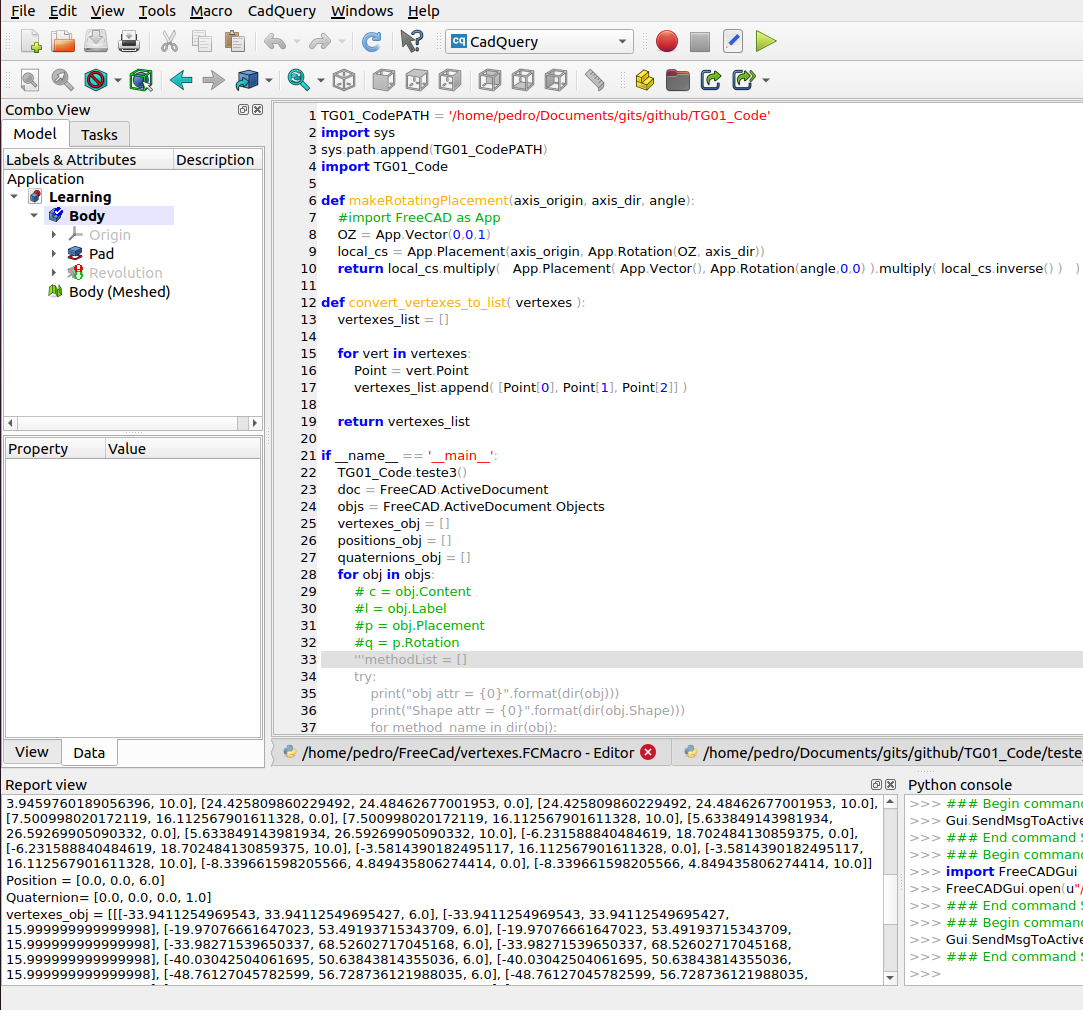
\includegraphics[scale=0.3]{Capitulos/Cap02_figs/FreeCad_Python.png}
    \caption{Exemplo da execução de um código de \textit{Python} no \textit{FreeCad}, onde se pega os vértices, posição e a rotação por \textit{quaternion} dos objetos da cena}
    \label{fig:Cap02_FreeCad_Python_01}
\end{figure}

\textit{FreeCad}, ao poder executar um \textit{script} que interage com os objetos da cena, permitindo acesso aos atributos listados abaixo:
\begin{itemize}
    \item \textit{Placement}: Objeto \textit{Python} que possui os valores associados a posição e rotação do modelo 3D.
    \begin{itemize}
        \item \textit{Base}: Objeto \textit{Python} que possui  posição (x, y, z).
        \item \textit{Rotation}: Objeto \textit{Python} que possui os valores da rotação do objeto, podendo adquirir a rotação por um Eixo, ou os valores em \textit{quaternion}.
    \end{itemize}
    \item \textit{Shape}: Atributo do objeto que possui informações da forma do modelo tridimensional, como os vértices e arestas.
    \begin{itemize}
        \item \textit{Vertexes}: É a lista dos vértices, que possuem o atributo \textit{Point} que é o valor das posições do vértice no eixo XYZ.
        \item \textit{Edges}: É a lista das arestas da forma tridimensional. 
    \end{itemize}
\end{itemize}

Assim garantindo que os dados dos objetos seja de fácil obtenção.

\section{\textit{C++}}
O \textit{C++} sera a ferramenta principal do trabalho, pois o código em \textit{C++} será o responsável por receber os dados brutos dos objetos da cena do \textit{FreeCad} como vértices, arestas, posições e rotação. Retornando as informações necessárias para que o \textit{FreeCad} reposicione os seus elementos na posição e rotação desejada. \newline
Dessa forma o código em \textit{C++} será responsável por:

\begin{enumerate}
    \item Pré-processamento: Os dados de posição e vértices de cada peça obtidos do \textit{FreeCad} vão ser armazenados por estruturas de dados do \textit{CGAL}\cite{cgal:complete_manual}, assim sendo projetados no plano XY, em seguida será determinado a forma poligonal a ser obtida usando o algoritmo do fecho convexo\cite{cgal:convex_hull}.
    \item Empacotamento: Usando um algoritmo genético para se determinar as posições e rotações dos polígonos, no qual seja encontrado uma solução para o problema proposto, podendo ser o de empacotar na menor areá retangular ou dentro de uma forma geométrica assim como \textit{knolling}.
    \item Pós-processamento: Uma forma de passar determinar a translação e rotação a ser realizada nas peças do \textit{FreeCad} para mostrar o empacotamento na cena.
\end{enumerate}

\subsection{\textit{CGAL}}

\cite{cgal:software} É uma sigla para \textit{Computational Geometry Algorithms Library}, em português significa Livraria de algoritmos de geometria computacional.\newline
\cite{cgal:complete_manual}\textit{CGAL} é um projeto de \textit{software} que provê algoritmos eficientes e confiáveis na forma de uma biblioteca de \textit{C++}.\textit{CGAL} é usado em varias áreas onde é necessário computações geométricas, como sistemas de informação geográfica, biologia molecular, imagens medica, computação gráfica e robótica.\newline

A biblioteca oferece estruturas de dados e algoritmos como triangulação, diagramas de Voronoy, operações boolianas com polígonos e poliedros, processamento de conjuntos de pontos, arranjos de curvas e superfícies, processamento de geometria, formas alfas, algoritmos de fecho convexo, entre outras funcionalidades. \newline

\cite{cgal:convex_hull}A função de fecho convexo tem sua funcionalidade que será utilizar os pontos projetados de cada objeto 3D para formar o seu respectivo polígono no plano XY, dessa forma pode-se determinar sobreposições, realizar translação e rotações dos polígonos, assim permitindo o uso do algoritmo genético para a solução do problema proposto na seção \ref{cap:introducao:sec:problema}.

\begin{figure}[H]
    \centering
    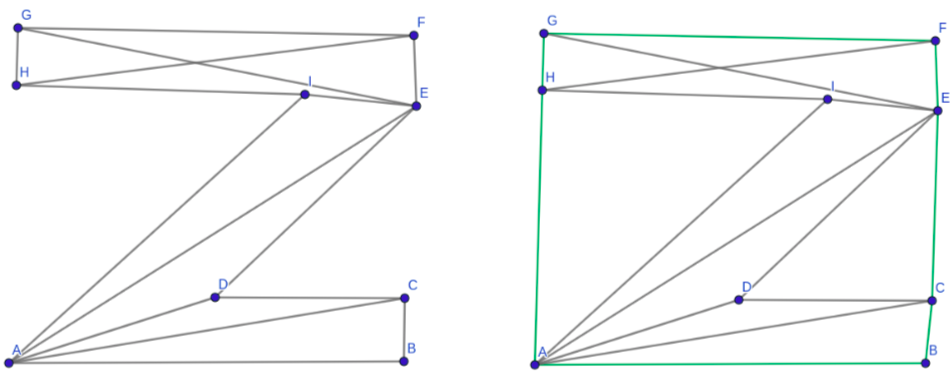
\includegraphics[scale=0.4]{Capitulos/Cap02_figs/CGAL_Convex_EX.png}
    \caption{Exemplo de um objeto projetado com suas arestas no plano XY, com os seus vértices sendo processados pela função do fecho convexo no lado direito, pode-se ver que nesse exemplo ocorre um consumo maior de espaço do que o necessário, devido ao fato do polígono a ser formado ter que ser convexo.}
    \label{fig:Cap02_CGAL_Convex_EX}
\end{figure}

Como para o problema de empacotamento, nos não queremos que ocorra sobreposição dos polígonos, logo será usado funções para se determinar intersecções entre os polígonos, assim influenciando na seleção do GA.

\subsection{\textit{Boost}}
\cite{boost:software} \textit{Boost} provê fontes de bibliotecas portáveis de \textit{C++} revisadas por pares.\newline
Enfatiza que as bibliotecas vão funcionar bem com a \textit{Standard Library} do \textit{C++}. As bibliotecas do \textit{Boost} são pensadas para terem um uso abrangente, e usabilidade para diversos tipos de aplicações. A licença do \textit{Boost} encoraja o uso de suas bibliotecas para todos os usuários com o mínimo de restrições.

\cite{boost:Python} A biblioteca \textit{Boost Python} é um \textit{framework} para fazer a interface entre \textit{Python} e \textit{C++}. O que permite uma forma simples e rápida de expor as classes, objetos e funções do \textit{C++} para o \textit{Python}, e vice-versa, sem a necessidade de ferramentas além do compilador de \textit{C++}. Ela é formulada para integrar \textit{C++} de forma não intrusiva, de tal modo que não seja necessário fazer qualquer alteração do código de \textit{C++}, fazendo \textit{Boost.Python} ideal para expor bibliotecas de terceiros ao \textit{Python}. A biblioteca usa técnicas avançadas de meta-programação para simplificar a sua sintaxe aos usuários, de forma que integrar o código toma uma forma de IDL declarativa.\newline
Assim será usada para integrar o código em \textit{Python} com o de \textit{C++}.

\cite{boost:dynamic_bitset}A classe \textit{dynamic\_bitset} representa um conjunto de bits. Este provê o acesso ao bit individualmente pelo operador [ ] e provê operadores de bits que só podem ser aplicados à inteiros nativos de \textit{C++}, como o operador \&. O número de bits pode ser especificado durante a execução como parâmetro do construtor do \textit{dynamic\_bitset}, o que o torna uma opção mais atrativa que o \textit{bitset} da \textit{Standard Library}, que tem o seu tamanho definido na compilação. Assim fazendo uma ótima estrutura de dados para os genes do GA.

% \cite{openapi:gen} apresenta uma vasta gama de geradores baseados na IDL OpenAPI. Até
% a presente data, apresenta 66 geradores de clientes para 33 linguagens e 41 geradores
% de servidores para 16 linguagens. Esse é o principal programa utilizado para gerar
% código em projetos que usam OpenAPI para especificação de suas APIs.

% Analisando o código-fonte e documentação do projeto, chegamos às seguintes conclusões:

% \begin{itemize}
% \item
%   Os geradores funcionam com base em um modelo genérico baseado em OpenAPI. O processo
%   de geração ocorre da seguinte maneira:

%   \begin{enumerate}
%   \item
%     O programa lê a especificação OpenAPI e a transforma no modelo genérico.
%   \item
%     A classe do gerador modifica esse modelo da forma que precisar, possivelmente
%     adicionando propriedades específicas para ele.
%   \item
%     O programa envia o modelo final para um motor de \textit{templates}, que
%     carrega os templates do gerador específico e os renderiza. O resultado dessa
%     etapa é o código final.
%   \end{enumerate}

%   Esse fato pode acabar por limitar a expressividade do gerador, pois o modelo
%   OpenAPI não é capaz de expressar, de forma simples, todos os detalhes envolvidos
%   em uma linguagem de programação.
% \item
%   Apesar de ser possível criar um novo gerador customizado, por exemplo, para uma
%   linguagem que o projeto não suporte, sem a necessidade de modificar o programa
%   em si, os geradores são estruturas monolíticas. Não é possível implementar uma
%   funcionalidade nova, e.g. um novo processo de validação, que possa ser usado por
%   todos os geradores. Isso limita significativamente a extensibilidade do projeto,
%   além de aumentar a carga operacional nessas situações.
% \end{itemize}

% \cite{googl:protobuf} é o compilador de Protocol Buffers. Ele apresenta uma estrutura
% bastante interessante em questão de extensibilidade: o sistema de \textit{plugins}.
% Um \textit{plugin} é um programa que recebe uma mensagem \texttt{CodeGeneratorRequest}
% como entrada e escreve na saída uma mensagem \texttt{CodeGeneratorResponse}. As
% definições dessas duas mensagens são apresentadas em \cref{lst:code-gen-req} e
% \cref{lst:code-gen-res}, respectivamente.

% \begin{listing}[ht]
% \caption{Especificação de \texttt{CodeGeneratorRequest}}
% \label{lst:code-gen-req}
% \begin{minted}{protobuf}
% message CodeGeneratorRequest {
%   repeated string file_to_generate = 1;

%   optional string parameter = 2;

%   repeated FileDescriptorProto proto_file = 15;

%   optional Version compiler_version = 3;
% }
% \end{minted}
% \end{listing}

% \begin{listing}[ht]
% \caption{Especificação de \texttt{CodeGeneratorResponse}}
% \label{lst:code-gen-res}
% \begin{minted}{protobuf}
% message CodeGeneratorResponse {
%   optional string error = 1;

%   message File {
%     optional string name = 1;

%     optional string insertion_point = 2;

%     optional string content = 15;
%   }

%   repeated File file = 15;
% }
% \end{minted}
% \end{listing}

% Esse sistema é interessante por dois fatores:

% \begin{itemize}
% \item
%   É muito simples adicionar suporte a uma nova linguagem, precisamos apenas
%   implementar um \textit{plugin}. Ponto em comum com o trabalho anterior.
% \item
%   Usando o campo \texttt{file.insertion\_point}, é possível injetar conteúdo
%   de um gerador em outro. O segundo gerador pode adicionar esses pontos no
%   arquivo gerado por ele, permitindo que outros geradores modifiquem o resultado
%   final.

%   Isso soluciona, em parte, o problema de adicionar novas funcionalidades em
%   um gerador presente em \cite{openapi:gen}. Dois problemas ainda persistem:

%   \begin{enumerate}
%   \item
%     Estamos limitados aos pontos de inserção disponibilizados pelo gerador, o
%     que pode variar de uma linguagem para outra. O quão grave é esse problema
%     depende do que se quer fazer com o \textit{plugin} e qual é a linguagem objeto.
%   \item
%     O sistema trabalha em termos de texto (campo \texttt{file.content}). Isso
%     limita o quão genérico nossa funcionalidade pode ser, e.g. um \textit{plugin} de
%     validação poderia ser genérico caso o resultado fosse mais estruturado.

%     Um exemplo de plugin que poderia ser genérico é \cite{envoy:protoc-gen-validate},
%     que provê uma extensão para diversas validações. Hoje, ela é limitada para
%     as linguagens Go, C++ e Java. Caso o resultado fosse mais estruturado, seria
%     possível implementar tal funcionalidade de forma genérica para uma grande
%     quantidade de linguagens.
%   \end{enumerate}
% \end{itemize}

% \cite{9159071} se propõe a resolver um problema diferente dos trabalhos anteriores:
% ele gera testes baseado em \textit{Property Based Testing} \cite{10.1145/351240.351266}
% a partir de especificações OpenAPI que validam que as respostas da API seguem as
% propriedades e formatos especificados. O programa é capaz de gerar esses testes
% sem a necessidade de nenhuma extensão a especificação.

% \cite{sferruzza:hal-01868498} propõe extensões e um gerador para OpenAPI que é
% capaz de modelar como uma operação é implementada. O trabalho cria o conceito de
% \textit{componentes atômicos e compostos}: componentes atômicos recebem parâmetros
% e podem gerar novos valores e componentes compostos fazem a composição de diversos
% componentes para definir uma dada lógica. O programa então é capaz de validar que
% as definições e uso dos componentes são válidas, tanto em questão de todas as
% variáveis estarem disponíveis quanto que os tipos estão corretos. O gerador é capaz
% de gerar código que define esses componentes.

% Por fim, \cite{r2c:semgrep} é uma ferramenta de análise estática que suporta uma
% quantidade impressionante de linguagens. O diferencial dessa ferramenta é que
% o usuário pode criar novas regras de análise utilizando uma DSL implementada sobre
% YAML, permitindo com que a mesma regra seja aplicada em diversas linguagens. Isso
% é possível pois todas as linguagens que ela suporta são convertidas para
% \textit{uma mesma linguagem intermediária} antes das regras serem aplicadas. Essa
% funcionalidade é similar a situação em que queremos implementar uma funcionalidade
% no nosso gerador de forma independente da linguagem objeto.
